\subsection{Imágenes satelitales}

Las imágenes satelitales son representaciones gráficas adquiridas mediante sensores ubicados en satélites que orbitan alrededor de la Tierra. Estos satélites, además de proveer imágenes, tienen una diversidad de aplicaciones, como la comunicación, la navegación, la investigación científica y la observación terrestre \cite{canada2007fundamentals}.

Dentro de los satélites empleados en teledetección, los más destacados son los satélites de observación \cite{canada2007fundamentals}. Estos están equipados con sensores que capturan información mediante la radiación electromagnética reflejada o emitida por la superficie terrestre y otros fenómenos atmosféricos. Además de los satélites de observación, existen otros que se dedican al monitoreo climático, posicionamiento (como los GPS), y estudios atmosféricos, por mencionar algunos \cite{jensen2016introductory}.

Cada imagen satelital se almacena en estructuras de datos multi dimensionales, comúnmente matrices, en donde cada elemento representa la información detectada por el sensor \cite{chuvieco2016fundamentals}. Dependiendo de la etapa de procesamiento en la que se encuentre la imagen, estos elementos pueden representar valores digitales, valores de radiancia o valores de reflectancia.

\subsubsection{Niveles de procesamiento}

Los niveles de procesamiento indican los tratamientos aplicados a la información originalmente capturada por el sensor. Estos procesamientos influencian en los valores registrados en la imagen satelital, que pueden categorizarse según su nivel de procesamiento, como se detalla en el Cuadro~\ref{tab:NivelProcesamientoImagenSatelital}.

\begin{table}[H]
    \caption{Niveles de procesamiento de una imagen satelital.}
    \begin{tabularx}{1\textwidth}{p{4cm}X}
        \hline
        \textbf{Nivel de  \newline procesamiento} & \textbf{Descripción}                                                                                                                                                                                                                                                                                                                                                                          \\
        \hline
        Valores Digitales                         & Representan los datos inalterados que provienen directamente del sensor, ya sea en un satélite o en una aeronave. Corresponden a la cantidad de energía electromagnética percibida por el sensor y convertida en un número digital, comúnmente en una escala de 0 a 255 para imágenes de 8 bits. No han sido sujetos a correcciones o calibraciones.                                          \\
        \hline
        Valores de radiancia                      & Denotan una medida física de la energía electromagnética que emana de una fuente y es detectada por el sensor satelital. Esta se expresa en términos de potencia por unidad de área y por unidad de ángulo sólido. Los valores digitales se pueden transformar a valores de radiancia usando coeficientes de calibración suministrados por las agencias encargadas de los satélites.          \\
        \hline
        Valores de reflectancia                   & Indican la proporción de energía solar que, tras incidir en la superficie terrestre, es reflejada de vuelta al sensor. Se representa típicamente como un valor entre 0 y 1 o en porcentaje. Para transformar los valores de radiancia a reflectancia es necesario considerar aspectos como la distancia Tierra-Sol al momento de la captura, el ángulo solar y las correcciones atmosféricas. \\
        \hline
    \end{tabularx}
    \begin{minipage}{\textwidth}
        \vspace{10pt}
        \reference{Datos tomados de \citeA{jensen2016introductory}.}
        \label{tab:NivelProcesamientoImagenSatelital}
    \end{minipage}
\end{table}

\subsubsection{Niveles de corrección}

Cada nivel de corrección aborda distintas imperfecciones o distorsiones que pueden haberse introducido en diferentes etapas del proceso de adquisición.

\textbf{a) Corrección radiométrica}

Se restauran aquellos píxeles que puedan haberse visto afectados durante el proceso de adquisición de datos. Algunos píxeles pueden haberse deteriorado o incluso perdido. Para contrarrestar esto, se recurre a técnicas que estiman valores a partir de promedios adyacentes u otros métodos similares. Una distorsión común es el bandeado, originado por discrepancias en la calibración entre detectores. La corrección del bandeado se basa en la hipótesis de que, en ausencia de errores, los histogramas de cada detector deberían ser consistentes entre sí y, simultáneamente, alinearse con el histograma global de la imagen \cite{jensen2016introductory}.

\textbf{b) Corrección geométrica}

Las imágenes son sometidas a un proceso de georreferenciación, asignando a cada píxel una coordenada geográfica específica \cite{chuvieco2016fundamentals}. No obstante, al realizar esta operación, pueden introducirse distorsiones. Para rectificar estas imprecisiones, se adoptan medidas como la corrección orbital, la identificación de puntos de control en tierra, el cálculo de errores por mínimos cuadrados, y la integración de modelos digitales de elevación \cite{jensen2016introductory}.

\textbf{b) Corrección atmosférica}

La corrección atmosférica busca identificar y rectificar las distorsiones provocados por la presencia gases y partículas, garantizando que la información registrada por el sensor refleje de manera más precisa las condiciones reales en la superficie terrestre \cite{bravo2017teledeteccion}. Estas correcciones se fundamentan en modelos atmosféricos y algoritmos que consideran la composición y condiciones de la atmósfera en el momento de la captura \cite{jensen2016introductory}.

\subsubsection{Índices espectrales}

\textbf{a) NDVI}

El NDVI (Índice de Vegetación de la Diferencia Normalizada) es utilizado para estimar la cantidad, calidad y desarrollo de la vegetación. Basándose en cómo la vegetación refleja la luz en distintas partes del espectro, especialmente en las bandas roja y NIR, el NDVI es una métrica de la actividad fotosintética y salud de la vegetación. Un NDVI positivo generalmente indica áreas vegetadas, mientras que valores negativos o cercanos a cero pueden representar áreas no vegetadas o vegetación estresada \cite{rouse1974monitoring}.

\begin{equation*}
    NDVI = \frac{NIR - Red}{NIR + Red}
\end{equation*}

\textbf{b) NDWI}

El NDWI (Índice de Agua de la Diferencia Normalizada) se utiliza ampliamente para monitorear el contenido de agua en la vegetación y para identificar masas de agua. La versión que utiliza las bandas Green y NIR es efectiva para detectar el contenido de agua en la vegetación. Otras variantes del NDWI que emplean la banda SWIR son más adecuadas para identificar cuerpos de agua, ya que esta banda es más sensible a cambios en el contenido de agua en el suelo \cite{gao1996ndwi}.

\begin{equation*}
    NDWI = \frac{Green - NIR}{Green + NIR}
\end{equation*}

\textbf{C) NDSI}

El NDSI (Índice de Nieve de la Diferencia Normalizada) se utiliza para identificar y monitorizar la cobertura de nieve en áreas terrestres. Este índice es útil en áreas polares o montañosas y es esencial para estudios climáticos, hidrológicos y de gestión del agua, ya que la nieve tiene un papel crítico en el balance hídrico de muchas regiones \cite{dozier1989spectral}.

\begin{equation*}
    NDSI = \frac{Green - SWIR}{Green + SWIR}
\end{equation*}

\subsubsection{Sentinel-2}

Las imágenes satelitales de Sentinel-2 son generadas a partir de los sensores ubicados en las plataformas Sentinel-2A, y Sentinel-2B. Ambos satélites forman parte del programa espacial Copernicus de la Agencia Espacial Europea (ESA), y fueron lanzados el 23 de junio de 2015 y el del Sentinel-2B respectivamente. El objetivo principal de Sentinel-2, es el seguimiento de la vegetación, la cobertura del suelo, y los recursos hídricos, además de la observación de cuerpos de agua interiores y zonas costeras \cite{sentinel2}.

\begin{figure}[H]
    \begin{center}
        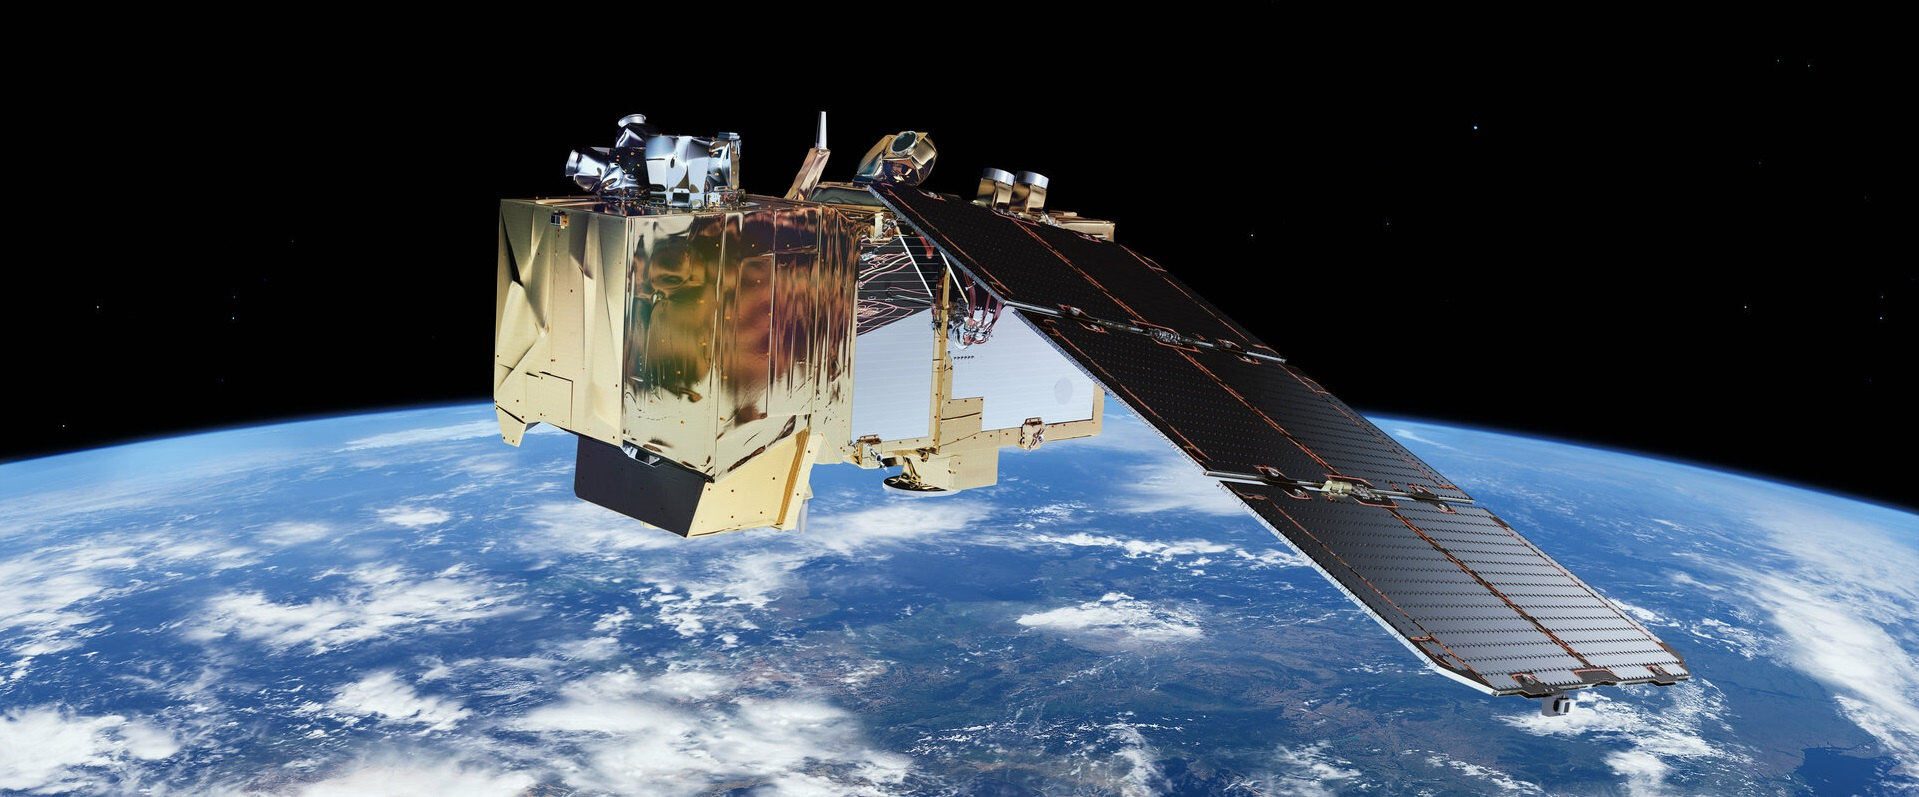
\includegraphics[width=1\textwidth]{Images/Sentinel2.jpg}
    \end{center}
    \caption{Plataforma Sentinel-2.}
    \reference{Datos tomados de \citeA{sentinel2}.}
    \label{fig:Sentinel2}
\end{figure}

Además de Sentinel-2, otras misiones espaciales relacionadas son Sentinel-1 y Sentinel-3. Sentinel-1 se compone de dos satélites, Sentinel-1A y Sentinel-1B (inoperativo), que cuentan con sensores activos, permitiendo la captura de datos independientemente del momento del día. Sentinel-1A fue puesto en órbita el 3 de abril de 2014. Con una frecuencia de adquisición de imágenes cada 6 días, estos satélites operan en la banda C y están orientados a ofrecer servicios terrestres y marinos. Algunas de sus aplicaciones incluyen el monitoreo de inundaciones, seguimiento de la superficie terrestre y análisis de patrones marinos.

Por otro lado, Sentinel-3, con sus satélites gemelos Sentinel-3A y Sentinel-3B, está equipado con una variedad de instrumentos: el Instrumento de Color Oceánico y Terrestre (OLCI), el Radiómetro de Temperatura de Superficie Terrestre y Marina (SLSTR), el Altímetro Radar SAR (SRAL) y el Radiómetro de Microondas (MWR). Estos instrumentos se enfocan tanto en el monitoreo marino como terrestre.

\textbf{a) Resoluciones}

Sentinel 2A y Sentinel 2B poseen características técnicas idénticas. Por este motivo, el Cuadro~\ref{tab:ResolucionesSentinel2} hace referencia a las resoluciones de ambos como Sentinel-2.

\begin{table}[H]
    \caption{Resoluciones de las imágenes Sentinel-2.}
    \small
    \begin{tabularx}{1\textwidth}{XX}
        \hline
        \textbf{Resolución}     & \textbf{Descripción}                                                                                                                                                                                                                                                                                    \\ \hline
        Resolución espacial     & La resolución espacial máxima de las imágenes Sentinel-2 es de 10 metros. No obstante, cada banda puede presentar una resolución espacial diferente, que puede ser de 10, 20 o 60 metros. Los detalles sobre la resolución espacial se encuentran especificados en el Cuadro~\ref{tab:BandasSentinel2}. \\ \hline
        Resolución espectral    & El sensor captura información en 13 bandas que abarcan desde el espectro visible e infrarrojo (VNIR) hasta el infrarrojo de onda corta (SWIR).                                                                                                                                                          \\ \hline
        Resolución radiométrica & Los productos obtenidos por el sensor, en términos de radiancia, poseen una resolución radiométrica de 12 bits (valores de píxeles de 0 a 4095). En contraste, los productos que representan la reflectancia se almacenan con números enteros de 16 bits.                                               \\ \hline
        Resolución temporal     & La resolución temporal de cada satélite es de 10 días, y la constelación combinada ofrece una resolución temporal de 5 días.                                                                                                                                                                            \\
    \end{tabularx}
    \begin{minipage}{\textwidth}
        \vspace{10pt}
        \reference{Datos tomados de \citeA{sentinel2}.}
        \label{tab:ResolucionesSentinel2}
    \end{minipage}
\end{table}

\textbf{b) Bandas}

Sentinel-2A y Sentinel-2B disponen de 13 bandas espectrales, es decir, se consideran como imágenes multiespectrales. Los detalles de cada banda se especifican en el Cuadro~\ref{tab:BandasSentinel2}.

\begin{table}[H]
    \caption{Información espectral de una imagen Sentinel-2.}
    \small
    \begin{tabularx}{1\textwidth}{p{6cm}XX}
        \hline
        \textbf{Banda}               & \textbf{Longitud de onda central (\textmu m)} & \textbf{Resolución espacial (m)} \\
        \hline
        Band 01: Coastal aerosol     & 0.443                                         & 60                               \\
        Band 02: Blue                & 0.490                                         & 10                               \\
        Band 03: Green               & 0.560                                         & 10                               \\
        Band 04: Red                 & 0.665                                         & 10                               \\
        Band 05: Vegetation Red Edge & 0.705                                         & 20                               \\
        Band 06: Vegetation Red Edge & 0.740                                         & 20                               \\
        Band 07: Vegetation Red Edge & 0.783                                         & 20                               \\
        Band 08: NIR                 & 0.842                                         & 10                               \\
        Band 8A: Vegetation Red Edge & 0.865                                         & 20                               \\
        Band 09: Water vapour        & 0.945                                         & 60                               \\
        Band 10: SWIR - Cirrus       & 1.375                                         & 60                               \\
        Band 11: SWIR                & 1.610                                         & 20                               \\
        Band 12: SWIR                & 2.190                                         & 20                               \\
        \hline
    \end{tabularx}
    \begin{minipage}{\textwidth}
        \vspace{10pt}
        \reference{Datos tomados de \citeA{sentinel2}.}
        \label{tab:BandasSentinel2}
    \end{minipage}
\end{table}

\textbf{c) Productos}

Los tipos de producto generados por Sentinel-2 se especifican en el Cuadro~\ref{tab:SentinelTipoProducto}.

\begin{table}[H]
    \caption{Tipos de productos disponibles en Sentinel-2.}
    \small
    \begin{tabularx}{1\textwidth}{XXXX}
        \hline
        \textbf{Nombre} & \textbf{Descripción de alto nivel}                                             & \textbf{Producción y distribución}            & \textbf{Tamaño}                \\ \hline
        Level-1B        & Radiancia, (TOA), en la geometría del sensor.                                  & Generación sistemática y distribución online. & 27 MB (cada 23x25 $km^{2}$)    \\
        Level-1C        & Reflectancia, (TOA), en la geometría cartográfica.                             & Generación sistemática y distribución online. & 500 MB (cada 110x110 $km^{2}$) \\
        Level-2A        & Reflectancia, (BOA), corregidas atmosféricamente en la geometría cartográfica. & Generación sistemática y distribución online. & 600 MB (cada 110x110 $km^{2}$) \\ \hline
    \end{tabularx}
    \begin{minipage}{\textwidth}
        \vspace{10pt}
        \reference{Datos tomados de \citeA{sentinel2}.}
        \label{tab:SentinelTipoProducto}
    \end{minipage}
\end{table}

Las imágenes L1C se encuentran ortorectificadas y con niveles de reflectancia superior a la atmósfera (TOA), mientras que las imágenes L2A se encuentran ortorectificadas y con noveles de reflectancia por debajo de la atmósfera (BOA). Es decir, las imágenes L2A presentan corrección atmosférica (ver Figura~\ref{fig:ComparacionBOATOA}).

\begin{figure}[H]
    \begin{center}
        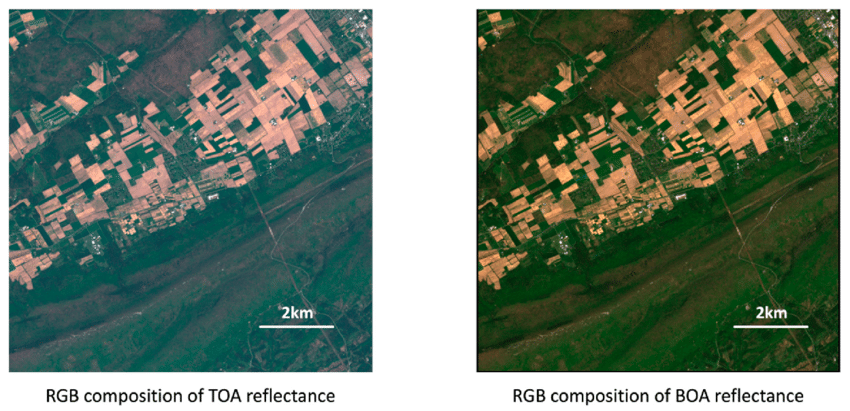
\includegraphics[width=1\textwidth]{Images/ComparacionBOATOA.png}
    \end{center}
    \caption{Comparación visual de dos imágenes (RGB) de Sentinel-2A: TOA, BOA.}
    \reference{Datos tomados de \citeA{song2020validation}.}
    \label{fig:ComparacionBOATOA}
\end{figure}

En el caso de las imágenes de nivel L1B, los productos se representan como ``gránulos'', los cuales abarcan un total de $23x25 km^2$ por cada uno. En el caso de las imágenes de nivel L1C y L2A, los productos representan ``mosaicos'', los cuales tienen un tamaño de $110x110 km^2$, los $10^2$ adicionales tienen el objetivo de evitar el solapamiento entre los mosaicos \cite{sentinel2}.

\subsubsection{Landsat}

Landsat es un programa de satélites de observación de la Tierra, el cual ha estado funcionando desde 1972 cuando se lanzó el primer satélite Landsat. Este programa es una colaboración entre la NASA y el USGS (Servicio Geológico de Estados Unidos)  \citeA{landsat}. La misión de Landsat es recopilar información sobre la superficie terrestre utilizando imágenes multiespectrales, proporcionando datos valiosos para la agricultura, cartografía, geología, silvicultura, planificación del uso del suelo y la educación, entre otras aplicaciones \cite{williams2006landsat}.


\begin{figure}[H]
    \begin{center}
        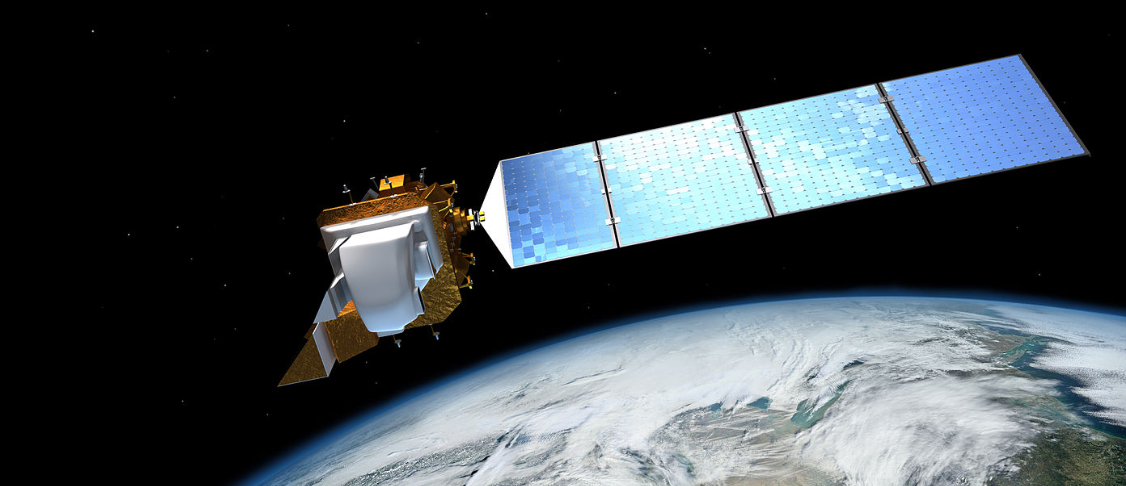
\includegraphics[width=1\textwidth]{Images/Landsat8.png}
    \end{center}
    \caption{Plataforma Landsat 8.}
    \reference{Datos tomados de \citeA{landsat}.}
    \label{fig:Landsat8}
\end{figure}

Los satélites Landsat recogen datos con resoluciones espaciales que pueden ser adecuadas para estudiar fenómenos a escala regional o global, y han sido fundamentales en el desarrollo de estudios sobre el cambio climático y la gestión de recursos naturales \cite{young2017land}. A lo largo de los años se han lanzado múltiples misiones Landsat. En el Cuadro~\ref{tab:ProgramaLandsat}, se detalla los años de lanzamiento y finalización de operaciones de cada satélite.

\begin{table}[H]
    \caption{Satélites del programa Landsat: Años de lanzamiento y finalización de operaciones.}
    \small
    \begin{tabularx}{1\textwidth}{p{2.5cm}p{5cm}X}
        \hline
        \textbf{Satélite Landsat} & \textbf{Año de lanzamiento} & \textbf{Año de finalización de operaciones} \\
        \hline
        Landsat 1                 & 1972                        & 1978                                        \\ \hline
        Landsat 2                 & 1975                        & 1982                                        \\ \hline
        Landsat 3                 & 1978                        & 1983                                        \\ \hline
        Landsat 4                 & 1982                        & 1993                                        \\ \hline
        Landsat 5                 & 1984                        & 2013                                        \\ \hline
        Landsat 6                 & 1993                        & Falló en alcanzar la órbita                 \\ \hline
        Landsat 7                 & 1999                        & Aún en operación                            \\ \hline
        Landsat 8                 & 2013                        & Aún en operación                            \\ \hline
        Landsat 9                 & 2021                        & Aún en operación                            \\ \hline
    \end{tabularx}
    \begin{minipage}{\textwidth}
        \vspace{10pt}
        \reference{Datos tomados de \citeA{landsat}.}
        \label{tab:ProgramaLandsat}
    \end{minipage}
\end{table}

\textbf{a) Resoluciones}

La resolución de un sensor montado en una plataforma Landsat varía según el satélite. A lo largo de las versiones de Landsat, se han producido cambios en la resolución y en las bandas espectrales de cada satélite. El Cuadro~\ref{tab:ResolucionLandsat} proporciona las especificaciones técnicas de las plataformas y sensores de los satélites Landsat.

\begin{table}[H]
    \caption{Información de las plataformas y sensores de los satélites Landsat.}
    \small
    \begin{tabularx}{1\textwidth}{YYYYY}
        \hline
        \textbf{Descripción}         & \textbf{Landsat 4} & \textbf{Landsat 5} & \textbf{Landsat 7} & \textbf{Landsat 8} \\ \hline
        Sensor                       & TM                 & TM                 & ETM+               & OLI/TIRS           \\ \hline
        Lanzamiento                  & 16/07/1982         & 01/03/1984         & 15/04/1999         & 11/02/2013         \\ \hline
        Altitud de órbita            & 705km              & 705km              & 705km              & 705km              \\ \hline
        Resolución Radiométrica      & 8bits              & 8bits              & 8bits              & 16bits             \\ \hline
        Resolución Espacial (metros) & 30m                & 30m                & 30m (B8 15m)       & 30m (B8 15m)       \\ \hline
        Resolución espectral         & 7 bandas           & 7 bandas           & 8 bandas           & 11 bandas          \\ \hline
        Resolución temporal          & 16 días            & 16 días            & 16 días            & 16 días            \\ \hline
        Tamaño de la imagen          & 180km x 180km      & 180km x 180km      & 180km x 180km      & 185km x 185km      \\ \hline
    \end{tabularx}
    \begin{minipage}{\textwidth}
        \vspace{10pt}
        \reference{Datos tomados de \citeA{bravo2017teledeteccion}.}
        \label{tab:ResolucionLandsat}
    \end{minipage}
\end{table}

\textbf{b) Bandas}

Las bandas espectrales en un satélite se refieren a los intervalos específicos del espectro electromagnético que el sensor es capaz de capturar \cite{chuvieco2016fundamentals}.

\begin{table}[H]
    \caption{Información espectral de una imagen Landsat 8.}
    \small
    \begin{tabularx}{1\textwidth}{p{6cm}XX}
        \hline
        \textbf{Banda}               & \textbf{Longitud de onda central (\textmu m)} & \textbf{Resolución espacial (m)} \\
        \hline
        Band 01: Coastal aerosol     & 0.433 – 0.453                                 & 30                               \\
        \hline
        Band 02: Blue                & 0.450 – 0.515                                 & 30                               \\
        \hline
        Band 03: Green               & 0.525 – 0.600                                 & 30                               \\
        \hline
        Band 04: Red                 & 0.630 – 0.680                                 & 30                               \\
        \hline
        Band 05: Near Infrared (NIR) & 0.845 – 0.885                                 & 30                               \\
        \hline
        Band 06: SWIR 1              & 1.560 – 1.660                                 & 30                               \\
        \hline
        Band 07: SWIR 2              & 2.100 – 2.300                                 & 30                               \\
        \hline
        Band 08: Panchromatic        & 0.500 – 0.680                                 & 15                               \\
        \hline
        Band 09: Cirrus              & 1.360 – 1.390                                 & 30                               \\
        \hline
        Band 10: Thermal 1           & 10.60 – 11.19                                 & 100                              \\
        \hline
        Band 11: Thermal 2           & 11.50 – 12.51                                 & 100                              \\
        \hline
    \end{tabularx}
    \begin{minipage}{\textwidth}
        \vspace{10pt}
        \reference{Datos tomados de \citeA{landsat}.}
        \label{tab:BandasLandsat8}
    \end{minipage}
\end{table}

Cada satélite Landsat tiene un conjunto particular de bandas diseñadas para observar características específicas en la superficie terrestre. Estas bandas se seleccionan en función de su utilidad para ciertas aplicaciones, como la observación de vegetación, agua, construcciones y otros elementos \cite{loveland2016landsat}. En función del número y tipo de bandas, los satélites Landsat pueden ser utilizados para una amplia gama de aplicaciones en teledetección.

El Cuadro~\ref{tab:BandasLandsat8} detalla las características de las bandas disponibles en el satélite Landsat 8 (ver Figura~\ref{fig:Landsat8}), que según \cite{hoeser2020object2}, es uno de los más empleados para tareas de teledetección.

\begin{figure}[H]
    \begin{center}
        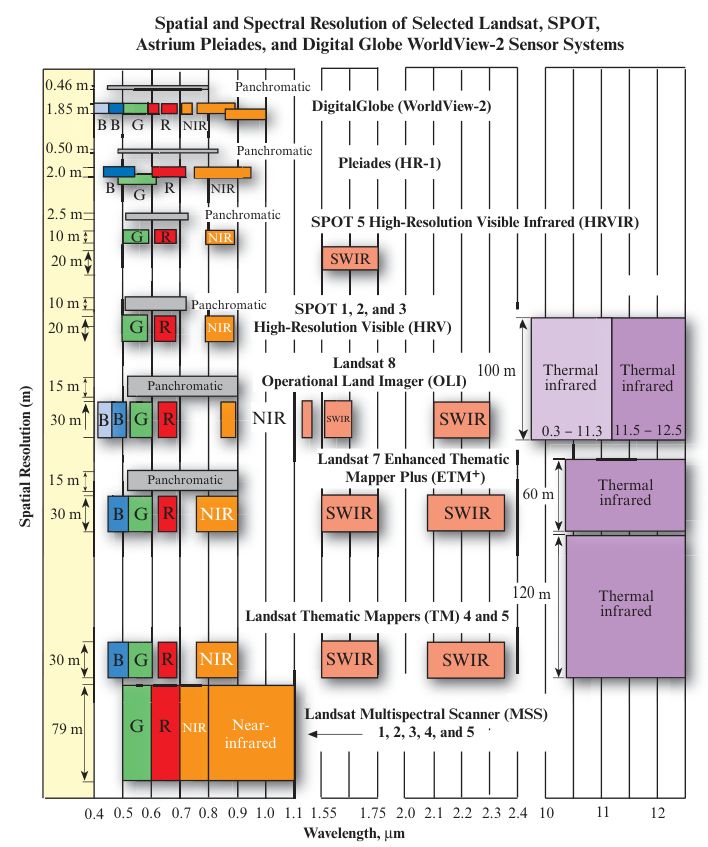
\includegraphics[width=1\textwidth]{Images/BANDAS.png}
    \end{center}
    \caption{Comparación de la distribución espectral entre los principales satélites de observación.}
    \reference{Datos tomados de \citeA{jensen2016introductory}.}
    \label{fig:BANDAS}
\end{figure}

En comparación con Sentinel-2, Landsat tiene la capacidad de obtener datos de la región térmica del espectro electromagnético, tal y como se ilustra en la Figura \ref{fig:BANDAS}. Esta característica permite recopilar información emitida directamente de la superficie terrestre. Landsat 8 cuenta con un sensor dedicado exclusivamente a esta área, el TIRS, mientras que el sensor OLI, está destinado a recopilar información de las demás regiones del espectro \cite{landsat}.

Landsat 8 ha aumentado su capacidad a aproximadamente 400 escenas diarias, superando las 250 escenas del Landsat 7 \cite{ariza2013descripcion}. Esto incrementa la probabilidad de obtener imágenes libres de nubes y aumenta la frecuencia de adquisición de datos \cite{loveland2016landsat}.

\textbf{c) Productos}

Según \citeA{ariza2013descripcion}, el formato GeoTIFF representa el estándar para la distribución de datos de Landsat, estando presente en los siguientes niveles de productos:

\begin{enumerate}
    \item \textbf{Nivel 0 (L0)}: Corresponde a las imágenes digitales crudas, sin procesar, que mantienen la secuencia de las bandas multiespectrales.

    \item \textbf{Nivel 1 Radiométrico (L1R)}: Incluye datos con correcciones radiométricas, ajustados a valores de radiancia o reflectancia espectral, derivados de datos de Nivel 0.

    \item \textbf{Nivel 1 Sistemático (L1G)}: Engloba los datos L1R con correcciones geométricas sistemáticas para el registro en una proyección cartográfica, utilizando como referencia el WGS84.

    \item \textbf{Nivel 1 Geométricamente corregido (L1Gt)}: Consiste en datos L1R con correcciones geométricas avanzadas, aprovechando información de posición a bordo y datos de control de elevación para corregir errores de paralaje.

    \item \textbf{Nivel 1 con Corrección del terreno (L1T)}: Agrupa los datos L1R con correcciones geométricas utilizando puntos de control terrestre y correcciones topográficas para contrarrestar el desplazamiento causado por el relieve.
\end{enumerate}